\section{Unscored competition inputs: coverage and disagreement}
\label{sec:evttc-competition}
\cohortline{UNSCORED INFERENCE / 434 query identities / 10 sequences / coverage and prediction disagreement}
We applied three released Garl-TTC variants to the same ten-sequence EvTTC inputs as the frozen PHASE-TTC reference. The 434 queries span eight road and two Slider sequences, with sequence, row, frame index, and timestamp matched across models. The comparison contains 1,302 Garl outputs and 434 PHASE-TTC outputs. \evidence{T01}

No verified numeric TTC targets map to these 434 query identities. We therefore measure coverage and paired prediction disagreement:
\begin{equation}
d_i^{(m)}=\widehat T_{i,m}^{\rm Garl}-\widehat T_i^{\rm PHASE},\qquad a_i^{(m)}=|d_i^{(m)}|.
\label{eq:evttc-disagreement}
\end{equation}
The differences in Equation~\ref{eq:evttc-disagreement} compare model outputs rather than prediction error. This population differs from both the labeled transfer in Section~\ref{sec:late-transfer} and Garl's published three-sequence RTE evaluation. Appendix~\ref{app:competition-details} gives the adapter, timing measurements, and ten sequence traces.

\subsection{Frozen checkpoints and native input support}
The released full, event-only, and visual-only state dictionaries load strictly and run in float32 with frozen weights. RGB-dependent routes use two real causal frames, while event-only uses two observed causal intervals. Startup queries without the required observations remain unavailable. PHASE-TTC uses up to 650\,ms of context, so the models share query identities under different temporal support. \evidence{T01}

Supplied boxes and calibration condition each route. Rotation-only projection omits translation because object depth is unavailable. For Slider, the adapter derives rotation from the supplied camera poses because the data provide no named event-to-RGB extrinsic. We treat the resulting runs as frozen-checkpoint adaptations.

\subsection{Coverage, sign, and disagreement tails}
\begin{table}[tbp]
\centering\small
\caption{Predictions on 434 EvTTC competition queries. The table reports finite-output coverage, signed TTC range, and negative counts. Median and P95 summarize absolute differences from PHASE-TTC where both models produce finite outputs. \evidence{T01}}
\label{tab:evttc-model-summary}
\begin{tabular}{@{}lrrrrr@{}}
\toprule
\textbf{Model} & \textbf{Finite} & \textbf{Range (s)} & \textbf{$<0$} & \textbf{Median (s)} & \textbf{P95 (s)} \\
\midrule
PHASE-TTC & 434/434 & [-42.225, 51.869] & 2 & -- & -- \\
Garl full & 424/434 & [0.907, 52.705] & 0 & 0.261 & 1.098 \\
Garl event-only & 434/434 & [-42.211, 406.095] & 10 & 0.681 & 5.623 \\
Garl visual-only & 426/434 & [-23.832, 38.767] & 5 & 0.236 & 1.524 \\
\bottomrule
\end{tabular}
\end{table}

PHASE-TTC and event-only Garl each emit 434 finite values; full Garl emits 424 and visual-only 426. The first query in each road sequence lacks two causal RGB frames, creating eight gaps in both RGB-dependent variants. Full Garl has two further Slider-750 gaps because the earlier event endpoint precedes recorded coverage. All invoked models return finite values; nulls correspond to unavailable inputs.

\begin{figure}[htbp]
\centering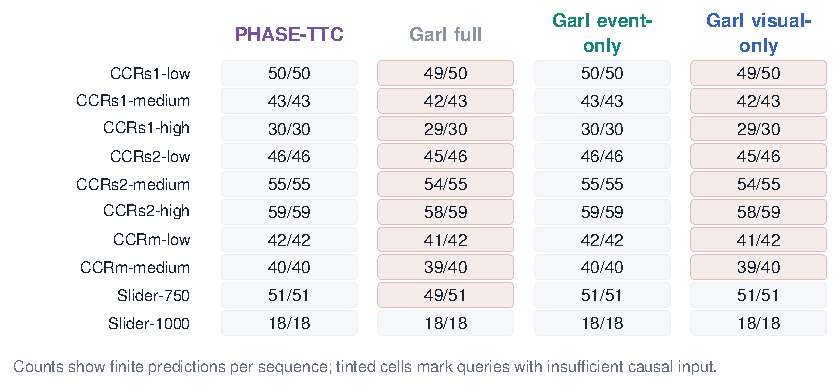
\includegraphics[width=\linewidth]{figures/rev_coverage.pdf}
\caption{\textbf{Finite prediction coverage by model and sequence.} Tinted cells mark the eight missing road RGB pairs and two additional early Slider-750 event gaps in full Garl. \evidence{T01}}
\label{fig:evttc-coverage}
\end{figure}

On shared finite rows, median absolute disagreement from PHASE-TTC is 0.26\,s for full Garl, 0.68\,s for event-only, and 0.24\,s for visual-only. Their p95 disagreements are 1.10, 5.62, and 1.52\,s. Full Garl emits no negative TTC, compared with two negative PHASE-TTC outputs, ten event-only outputs, and five visual-only outputs. \evidence{T01}

Slider-750 contains the largest excursions: event-only reaches 406.10\,s, with p95 absolute disagreement of 241.68\,s. The native height-ratio conversion becomes ill-conditioned as the two predicted endpoint heights approach equality. Figures~\ref{fig:evttc-predictions-symlog} and~\ref{fig:evttc-predictions-linear} preserve the sign and magnitude of these outputs across all ten sequences. \evidence{T01}

Timing remains descriptive because the variants ran once in fixed order with shared cache and warm-state effects, and PHASE-TTC used a different adapter and longer history. \evidence{T01}
\FloatBarrier
